\documentclass[paper=a4, fontsize=12pt]{scrartcl} % A4 paper and 11pt font size

\usepackage[T1]{fontenc} % use 8-bit encoding that has 256 glyphs
\usepackage{fourier}     % use the Adobe Utopia font for the document
                         % (comment this line to return to the LaTeX default)
\usepackage[english]{babel} % English language/hyphenation
\usepackage{amsmath,amsfonts,amsthm} % math packages
\usepackage{subeqnarray}

\usepackage{lipsum} % used for inserting dummy 'Lorem ipsum' text into the template
\usepackage{bold-extra}
\usepackage{enumitem}   
\usepackage{graphicx}
\usepackage{subcaption}
\usepackage{tcolorbox}
\usepackage{hyperref}




\usepackage{listings}
\usepackage[utf8]{inputenc}

% default fixed font does not support bold face
\DeclareFixedFont{\ttb}{T1}{txtt}{bx}{n}{12} % for bold
\DeclareFixedFont{\ttm}{T1}{txtt}{m}{n}{12}  % for normal

% custom colors
\usepackage{color}
\definecolor{deepblue}{rgb}{0,0,0.5}
\definecolor{deepred}{rgb}{0.6,0,0}
\definecolor{deepgreen}{rgb}{0,0.5,0}
\definecolor{lightblue}{rgb}{0.95,0.95,1}
\definecolor{lightgrey}{rgb}{0.6,0.6,0.6}
\usepackage{listings}

% use graphics packages
\usepackage{graphicx}
\usepackage{float}
\usepackage{tikz}
\usetikzlibrary{matrix}
\usetikzlibrary{calc}
\usetikzlibrary{patterns,fadings}

% python style for highlighting
\newcommand\pythonstyle{\lstset{
language=Python,
backgroundcolor=\color{lightblue},
basicstyle=\ttm,
otherkeywords={self,def},             % add keywords here
keywordstyle=\ttb\color{deepblue},
emph={while,for,if,elif,else,def,as,shape,conj,dot,copy,flatten,eye,zeros,ones,hstack,vstack,real,imag,conjugate,sin,cos,exp,append,insert,index,__main__}, % custom highlighting
%emphstyle=\ttb\color{deepred},     % custom highlighting style
emphstyle=\ttb\color{deepblue},     % custom highlighting style
stringstyle=\color{deepgreen},
commentstyle=\color{lightgrey},
frame=tb,                         % any extra options here
numbers=left,
showstringspaces=false            %
}}

% python environment
\lstnewenvironment{python}[1][]
{
\pythonstyle
\lstset{#1}
}
{}

% python for external files
\newcommand\pythonexternal[2][]{{
\pythonstyle
\lstinputlisting[#1]{#2}}}

% python for inline
\newcommand\pythoninline[1]{{\pythonstyle\lstinline!#1!}}


\usepackage{sectsty}        % allows customizing section commands
\allsectionsfont{\centering \normalfont\scshape}      % make all sections centered
                                                      % the default font and small caps

\usepackage{fancyhdr}        % custom headers and footers
\pagestyle{fancyplain}       % makes all pages in the document conform to
                             % the custom headers and footers
\fancyhead{}                 % no page header - if you want one, create it in
                             % the same way as the footers below
\fancyfoot[L]{}              % empty left footer
\fancyfoot[C]{}              % empty center footer
\fancyfoot[R]{\thepage}      % page numbering for right footer
\renewcommand{\headrulewidth}{0pt}     % remove header underlines
\renewcommand{\footrulewidth}{0pt}     % remove footer underlines
\setlength{\headheight}{13.6pt}        % customize the height of the header

\numberwithin{equation}{section}       % number equations within sections
                                       % (i.e. 1.1, 1.2, 2.1, 2.2 instead of 1, 2, 3, 4)
\numberwithin{figure}{section}         % number figures within sections
                                       % (i.e. 1.1, 1.2, 2.1, 2.2 instead of 1, 2, 3, 4)
\numberwithin{table}{section}          % number tables within sections
                                       % (i.e. 1.1, 1.2, 2.1, 2.2 instead of 1, 2, 3, 4)

\setlength\parindent{0pt}         % removes all indentation from paragraphs
                                  % comment this line for an assignment with lots of text

%--------------------------
%	TITLE SECTION
%--------------------------

\newcommand{\horrule}[1]{\rule{\linewidth}{#1}} % create horizontal rule command
                                                % with 1 argument of height

\title{
\normalfont \normalsize
\textsc{Imperial College London, Department of Mathematics} \\ [25pt]
\horrule{0.5pt} \\[0.4cm]                      % thin top horizontal rule
\huge Scientific Computing (M3SC) \\           % the assignment title
\horrule{2pt} \\[0.5cm]                        % thick bottom horizontal rule
}

\author{YOUR NAME\\
  YOUR CID}
\date{\normalsize\today}

\begin{document}
%\ttfamily
%\fontseries{b}\selectfont

\maketitle

\section*{Image Blending and Fractal Growth- Course Work}

In this coursework we will guide you through the development of an image blending algorithm and a fractal growth solver. 
Your submission must consist of ONE zip folder containing:

\begin{itemize}
\item 1 pdf report - using the LaTeX template provided on BB.
\item 2 Folders,  one for each part (Blending \& Fractals)
\begin{itemize}
\item Folder 1: ImBlending.py + 3 given images (source, mask, destination) + the 10 images required in the report.
\item Folder 2: Fractals.py  + 5  images required in the report  
\end{itemize}
\end{itemize}

\textbf{It is important that you get the results right, but this CW, more than the first one, will penalise inefficient and cumbersome codes. Speed is a priority here.}\\
\textbf{Do not modify any of the functions that are already provided}. If we cannot run your codes from our main script  you will lose marks. \\
\textbf{You are also advised to use the LaTeX template provided.}



\newpage
\section{ PART A:Image Blending (11 pts)}

This section will guide you through the development of a  image blending code. You are asked to apply the algorithm to a given example and to also generate your own image. The algorithm is based on the Poisson equation with Dirichlet boundary conditions applied to the region of the destination image you have to reconstruct with the source image.\\
The code you are given works on a  black and white image. You will modify it later on to handle colour images.
You should read or look at this paper:
\url{https://www.cs.virginia.edu/~connelly/class/2014/comp_photo/proj2/poisson.pdf}


\begin{align}
&\nabla^2 f= \nabla \cdot v  & \text{on } \Omega, \\ \notag
& f=g &  \text{on } \partial \Omega \\ \notag
\end{align}

\subsection{The neighbours [3 pts]}
The first task is to develop the function `Neighbours' which finds the indices of the masked area and their neighbours defined by the image mask.jpg. The nodes to be found are:

\begin{itemize}
\item The nodes of the masked area [Ic] (`Index centre')
\item Their northern neighbours [In]
\item Their southern neighbours [Is]
\item Their eastern neighbours [Ie]
\item Their western neighbours [Iw]
\end{itemize}

You will group the indices in a list called `Neigh' which is the output of the function. 
\begin{python}
def Neighbours(msk):
# msk:= binary matrix (only 0 & 1)
# Output---
# Neigh:=  list containg all the indices 
   
    Neigh=[Ic, In, Is, Iw, Ie]
    return Neigh
\end{python}
Test your function on the example shown in figure \ref{fig:table} and check that you obtain the following: \\

\begin{tabular}{ l | c }
  \hline
Ic& 9, 10, 11, 17, 18, 23, 24, 25, 26, 29, 30, 31, 32, 33, 38, 40\\
In&8,  9, 10, 16, 17, 22, 23, 24, 25, 28, 29, 30, 31, 32, 37, 39 \\
Is&10, 11, 12, 18, 19, 24, 25, 26, 27, 30, 31, 32, 33, 34, 39, 41\\
Iw&2,  3,  4, 10, 11, 16, 17, 18, 19, 22, 23, 24, 25, 26, 31, 33\\
Ie&16, 17, 18, 24, 25, 30, 31, 32, 33, 36, 37, 38, 39, 40, 45, 47\\
\hline  
\end{tabular}
\begin{figure}[H]
    \centering
        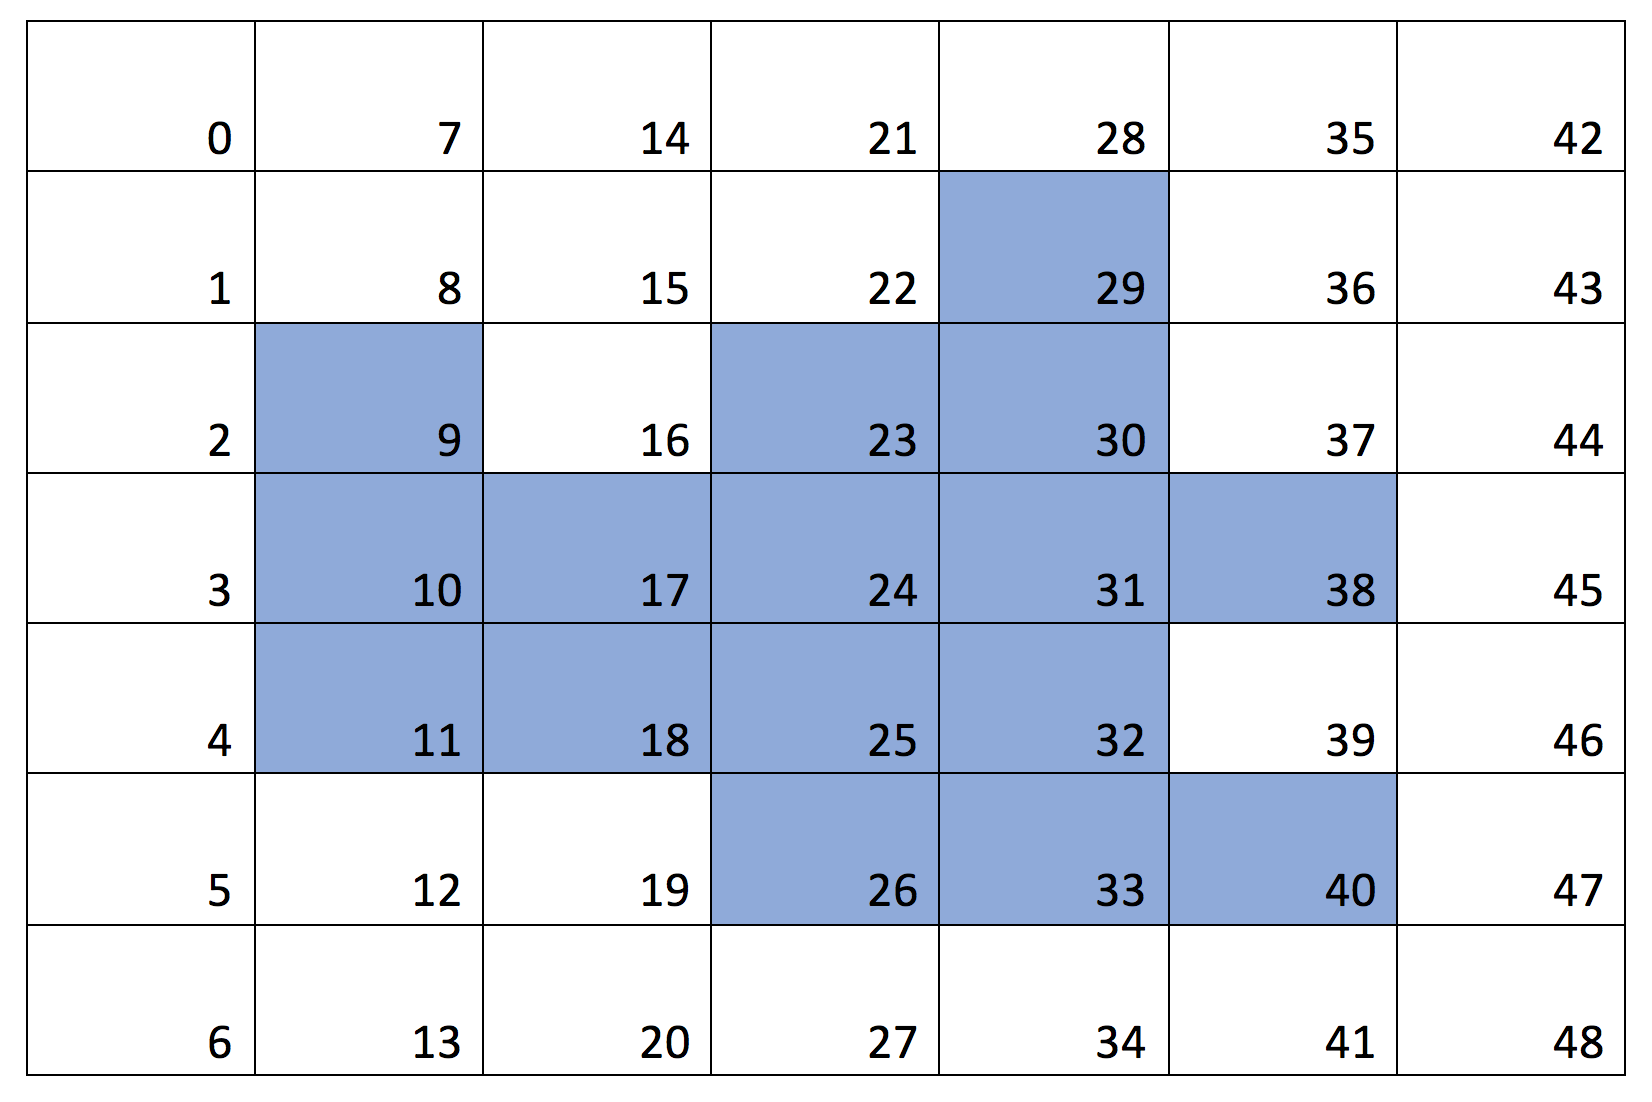
\includegraphics[width=.5\textwidth]{Table}
    \caption{Example nodes on the masked area}
    \label{fig:table}
\end{figure}

\textbf{NB if you numbered differently, remake this example with your numbering system and include it in the report. }


\subsection{Assembling the Discrete Laplace [5 pts]}
In this section you will assemble the Discrete Laplace operator for the unknown points and the boundary condition vector. This is done in the discretisation function `DiscFun' which takes as inputs the list Neigh from the previous function and the destination image `f'.  The first output is the discretisation matrix `D' which has `4'  on the point corresponding to the Ic indices, and `-1' on each entry corresponding to an unknown neighbour (In, Is, Iw, Ie). The second output is the $( n \times m, 1)$ vector that contains the boundary values of those neighbours that are outside the unknown area. \\
Make sure that the discrete Laplacian is now solved only in the masked domain ( points 0-15 as highlighted in red in figure \ref{fig:tab2}). \\
A way to do this is as follows:\\

1) Convert the indices Ic, In, Is, Ie, Iw to the domain numbering.  e.g. $9\rightarrow 0$, $10\rightarrow1$....\\
2) If an index is the boundary, then allocate the correct value in the rhs vector of boundary conditions.\\

Once you have those lists, assembling the matrix should be straight forward.\\
Make sure to implement this efficiently and with the ability to handle very large sizes.\\
Test that you can produce the right matrix for the small example.

\begin{figure}[H]
    \centering
        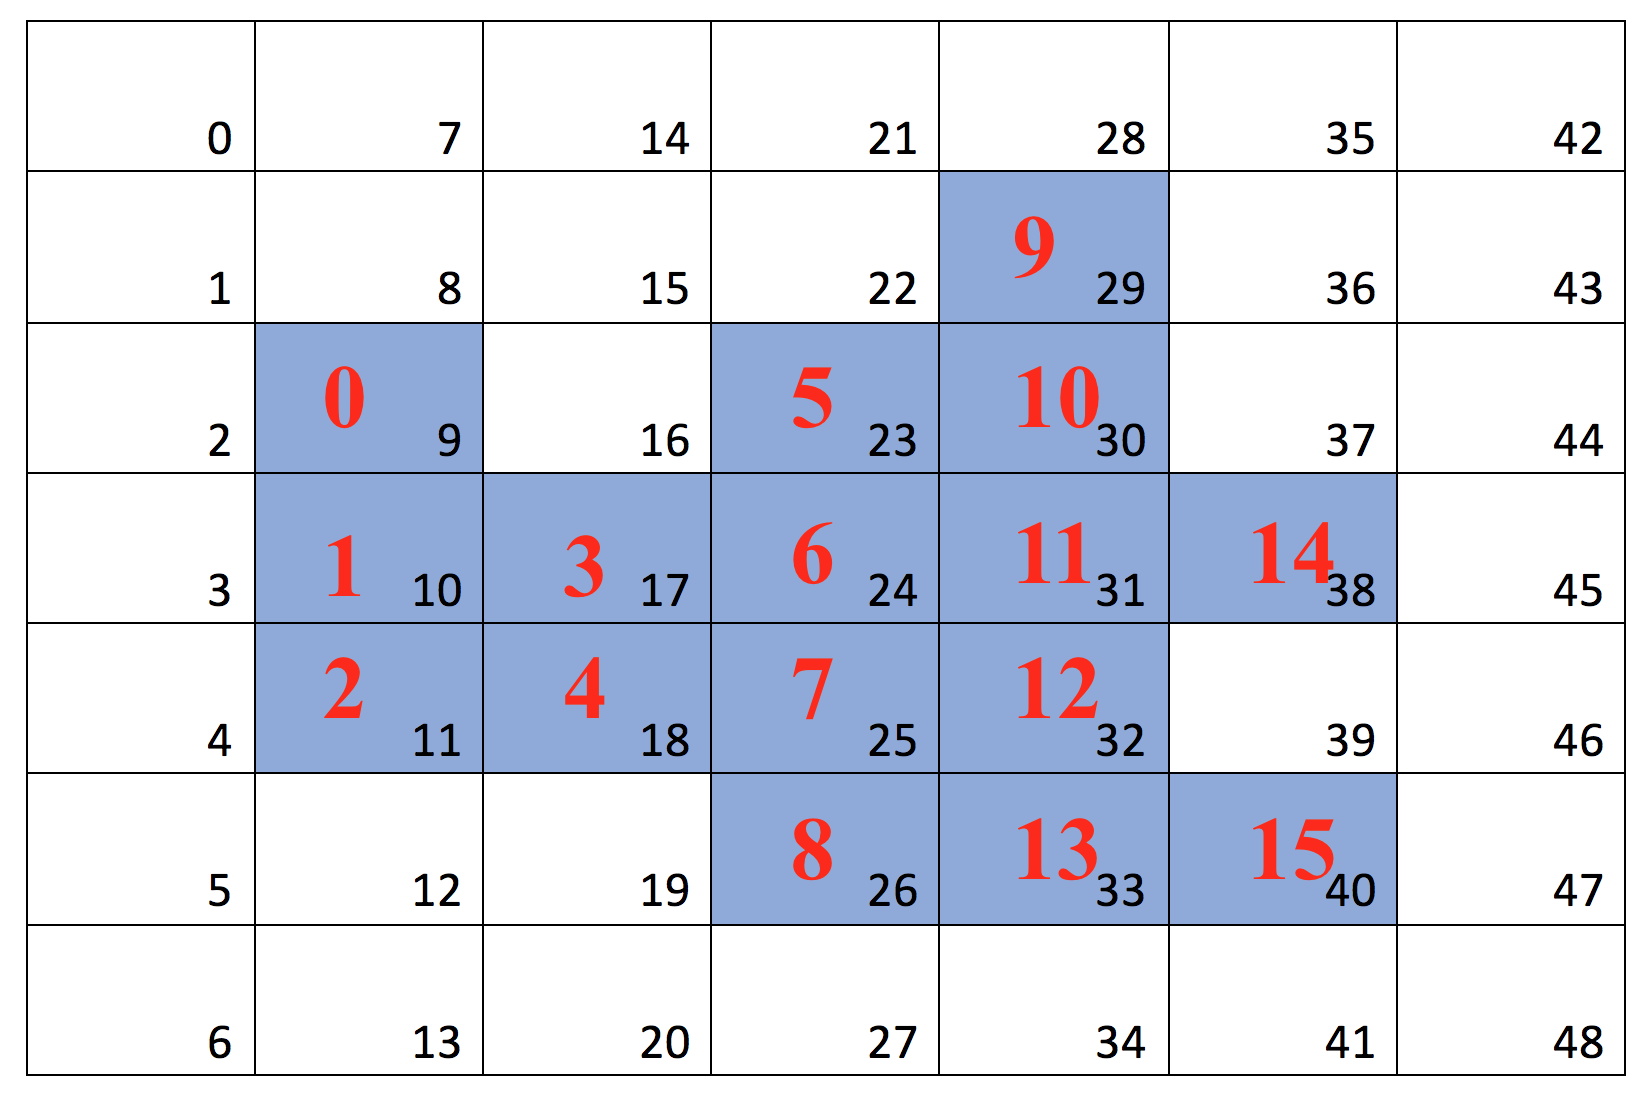
\includegraphics[width=.5\textwidth]{Table_index}
    \caption{Example nodes of the domain}
    \label{fig:tab2}
\end{figure}

\begin{python}
def  DiscFun( Neigh, f):
# Neigh from previous function
# f:= f^* (destination image)
# Output---
# D:= Discretization matrix
# bc:= rhs vector of the boundary values

# First convert Neigh to the new index list

# then assemble matrix and BC        
    return D, bc
 
\end{python}



Produce your first image by solving the problem with $v=0$  hence, only determined by the boundary conditions. Save your image in the first subplot of figure \ref{fig:1}.

\subsection{ Guiding gradients [0.5 pts]}
 Write the form of equation 1.1 if we use $v$ as the gradient of some scalar field $ \phi$. Obtain the right hand side (RHS) of equation 1.1 when we use  $\phi$ as the source image $g$  and destination image $f^*$.
 Embed the lines of code you used to generate the RHS. 
 Plot the normalised fields multiplied by a factor of 10 (This is only necessary to plot them, as the gradients are quite weak)
\begin{figure}[H]
    \centering
    \begin{subfigure}[b]{0.45\textwidth}
        
\includegraphics[width=\textwidth]{sample}
        \caption{ Guiding gradient destination image}
    \end{subfigure}
    \begin{subfigure}[b]{0.45\textwidth}
        
\includegraphics[width=\textwidth]{sample}
        \caption{Guiding gradient source image}
    \end{subfigure}
    \caption{Guiding gradients}
\end{figure}

 \begin{tcolorbox}
 
\begin{python}
#your few lines
\end{python}
 \end{tcolorbox}
 


\subsection{Source guiding gradient [0.5 pts]}
Having obtained the guiding gradient of the source image $g$, how do you modify the previous code to include the guiding gradient of the source image $g$ ? Plot the result  of solving eq. 1.1. in the second subplot of figure \ref{fig:1}.

 \begin{tcolorbox}
\begin{python}
# few lines
\end{python}
 \end{tcolorbox}
 
 What happens to the solution if you use the destination image $f^*$ as a  guiding gradient?
  \begin{tcolorbox}
1 line answer
 \end{tcolorbox}
 
 
 
 \subsection{Mixed guiding gradient [0.5 pts]}
How do you implement a mixed guiding gradient? where you take:

\begin{equation}
v=
\begin{cases}
\nabla f^* & \text{if } |\nabla f^*|>|\nabla g|\\
\nabla g& \text{otherwise}
\end{cases}
\end{equation}


 \begin{tcolorbox}
\begin{python}
your code (you may want to write a function for this)
\end{python}
 \end{tcolorbox}
 
 Produce the resulting image and place it in subplot 3 of figure \ref{fig:1}. 
  
 \subsection{An RGB image [0.5 pts]}
 How do you modify the algorithm to apply it to a colour image?
Show your result for a mixed guiding gradient in subplot 4 of figure \ref{fig:1}.

 \begin{tcolorbox}
Answer
\begin{python}
# few important lines,I will check the main function
\end{python}
 \end{tcolorbox}


\begin{figure}[H]
    \centering
    \begin{subfigure}[b]{0.45\textwidth}
        
\includegraphics[width=\textwidth]{sample}
        \caption{ Boundary only result}
    \end{subfigure}
    \begin{subfigure}[b]{0.45\textwidth}
        
\includegraphics[width=\textwidth]{sample}
        \caption{ Source guiding gradient}
    \end{subfigure}
    \begin{subfigure}[b]{0.80\textwidth}
        
\includegraphics[width=\textwidth]{sample}
        \caption{ Strongest Gradient}
    \end{subfigure}
        \begin{subfigure}[b]{0.80\textwidth}
        
\includegraphics[width=\textwidth]{sample}
        \caption{ Colour result}
    \end{subfigure}
    \caption{Your answer}
    \label{fig:1}
\end{figure}



 \subsection{Impress us [0.5 +0.5]}
 Apply the algorithm developed or a different type of RHS to an example of your choice, we will give 0.5 extra mark for going above and beyond the class material.  Plot together the source, mask, destination and final image. 
 You might find useful the provided scripts Masking.py  and roipoly.py that will help you generate the mask for an image (read the \textit{README} file before using them). Otherwise develop your own mask and way to adjust it. 

\begin{figure}[H]
    \centering
    \begin{subfigure}[b]{0.40\textwidth}
        
\includegraphics[width=\textwidth]{sample}
        \caption{ Source}
    \end{subfigure}
        \begin{subfigure}[b]{0.40\textwidth}
        
\includegraphics[width=\textwidth]{sample}
        \caption{ Mask}
    \end{subfigure}
    \begin{subfigure}[b]{0.40\textwidth}
        
\includegraphics[width=\textwidth]{sample}
        \caption{ Destination}
    \end{subfigure}
    \begin{subfigure}[b]{0.70\textwidth}
        
\includegraphics[width=\textwidth]{sample}
        \caption{ Final result}
    \end{subfigure}
    \caption{Your answer}
    \label{fig:1}
\end{figure}

\newpage
\section{SECTION B: Fractal Growth [9 pts]}
In this section you will develop a code to simulate  fractal growth. It is based on the steady state solution of the Fick's equation  augmented by a stochastic element.  We suggest you to make use of the function(s) developed in PART A. If you use those functions as they are, you don't need to show them again, just show how you use them.

You will grow the fractal in a 256$\times$ 256 unit square domain starting from a seed in the middle.
The equation you solve is given by the following:

\begin{align}
&\nabla^2 f= 0 & \text{on } \Omega, \\ \notag
& f=1 &  \text{on } \partial \Omega_f \\ \notag
& f=g(r) &  \text{on } \partial \Omega_b \\ \notag
\end{align}

where the boundary on the fractal edges are denoted by $\partial \Omega_f$ and the box boundaries are $ \partial \Omega_b$.  $g(r)$ is a function of the distance between the fractal and the edge ($r$) but for the first part of the problem take $g(r)$=0 on all the  box boundaries.



\subsection{The domain [0.5 pts] }
Use the function `Neighbours' from the previous part to obtain the domain in which you will solve the Laplace equation (2.1).  

 \begin{tcolorbox}
  Explain how you use it 
\begin{python}
# explain what is the input matrix
# one line to call the function
\end{python}
 \end{tcolorbox}


\subsection{The solution in the domain [0.5 pts] }
Use the previous function to obtain the discretisation matrix D and the boundary conditions to solve problem of equation 2.1 in the domain obtained from the previous point. 

 \begin{tcolorbox}
  Explain how you use it 
\begin{python}
# explain what is the input matrix
# one line to call the function
\end{python}
 \end{tcolorbox}

\subsection{The Neighbours of the fractals [1 pts] }
How can you obtain the indices of the neighbouring cells of the fractals? How do you obtain the value of the potential field for these cells?


 \begin{tcolorbox}
 Explain if you use previous functions
\begin{python}
#  lines of code

\end{python}
 \end{tcolorbox}



\subsection{Deposition [4 pts]  }
You will deposit a new seed in the neighbour specified by the algorithm explained in class. Complete the function `Deposition' such that it returns the index of the location where the new seed has to be placed.  


 \begin{tcolorbox}
\begin{python}
def Deposition(IB, p, alpha):
    
    # IB := indices of the neighbours of the fractals
    # p:= solution field everywhere
    #alpha := exponent
    # outputs:---
    # Idx := index to place next particle

    return Idx 
\end{python}
 \end{tcolorbox}
 



%You will:\\
% 
% Normalise  the values of the potential field $v$ according to $u_i=\frac{u_i^{\alpha}}{\sum(u_i^{\alpha})}$ for $i$ in the neighbours of the existing fractal.\\
% 
% Generate the cumulative sum of each cell and pick the one that is higher or equal to a  randomly generated number form a uniform distribution between 0 \& 1.
 
 \subsection{Fractal growth [1 pts] }
Add the seed to the  location given by `Idx' from the previous function and repeat the routine until one of the seeds is deposited on the boundaries. Produce 2 plots, one with $\alpha=1$ and one with $\alpha=3/2$.
How long did your code take to run?
 \begin{tcolorbox}
 .... minutes
 \end{tcolorbox}

 \subsection{Boundaries [0.5 pts]  }
Change the boundary conditions on the box such that they are:
\begin{equation}
 g(r)=\frac{1}{2 \pi}\ln(r)
\end{equation}
where $r$ is simply the distance from the centre of your square. 

Produce the results for 4000 iterations.
How long did your code take to run?


 \begin{tcolorbox}
 .... minutes
 \end{tcolorbox}
 
  \subsection{Impress us [0.5 pts]  }
  Make up your own fractal. Change boundaries and/or seeds and produce a cool fractal. Describe what you did.
 

\begin{figure}[H]
    \centering
    \begin{subfigure}[b]{0.49\textwidth}
        
\includegraphics[width=\textwidth]{sample}
        \caption{Fractals $\alpha=1$}
    \end{subfigure}
    \begin{subfigure}[b]{0.49\textwidth}
        
\includegraphics[width=\textwidth]{sample}
        \caption{Fractals $\alpha=3/2$}
    \end{subfigure}
    \caption{Your answer}
\end{figure}

\begin{figure}[H]
    \centering
    \begin{subfigure}[b]{0.49\textwidth}
        
\includegraphics[width=\textwidth]{sample}
        \caption{Fractals $\alpha=1$}
    \end{subfigure}
    \begin{subfigure}[b]{0.49\textwidth}
        
\includegraphics[width=\textwidth]{sample}
        \caption{Fractals $\alpha=3/2$}
    \end{subfigure}
    \caption{Your answer}
\end{figure}

\begin{figure}[H]
    \centering
        
\includegraphics[width=.8\textwidth]{sample}
    \caption{Your fractal}
\end{figure}

  \end{document}